% ANTENNE
De te ontwerpen antenne is een dipoolantenne geprint op een Printed Circuit Board (PCB), waarvan de
  lay-out in \cite{lesWendy} gegeven werd en die weergegeven is in figuur \ref{fig:antenne}. Van de
  aangeduidde waarden zijn de volgende gegevens reeds gekend:
  \begin{itemize}
    \item $Z_{AE} = 73 \Omega$
    \item De lengte van een tak van de antenne $L_{AE} = \frac{\lambda}{4}$
    \item De breedte van de dipool $W_{AE} = 6 \mbox{mm}$ volgens \cite{lesWendy}
    \item De lengte van de balun $L_b = \frac{\lambda}{4}$
    \item De karakteristieke impedantie van de microstriplijn $Z_{\mu} = 50 \Omega$.
  \end{itemize}
  
    \begin{figure}
      \centering
      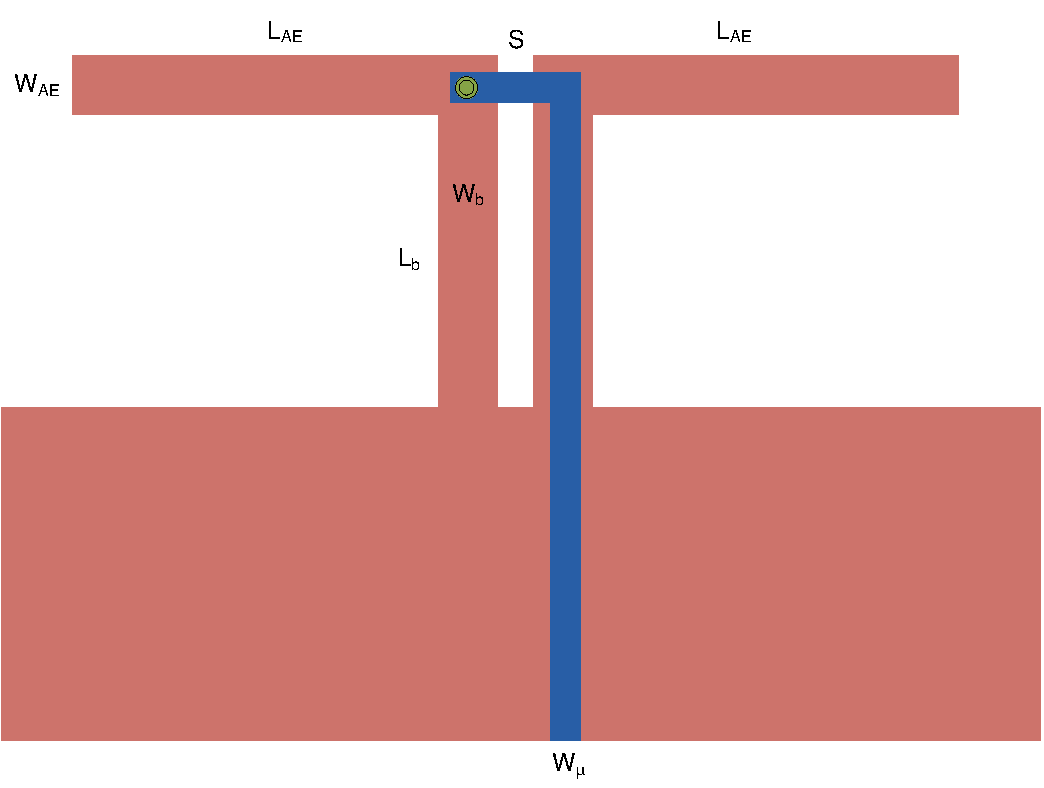
\includegraphics[width=0.7\textwidth,keepaspectratio=true]{fig/antenna.pdf}
      \caption{Geometrie antenne}
      \label{fig:antenne}
    \end{figure}

\section{Dipool}
Met behulp van WCalc \cite{Wcalc} worden de dimensies van de dipoolantenne bepaald.

  
    
  

\section{Balun}
Voor de balun worden de dimensies $W_b$, $L_b$ en $S$ bepaald via het model van
een gekoppelde microstriplijn in \cite{Wcalc} zoals uitgelegd in \cite{Edward}

\section{Lay-out}

\section{Metingen}


\tbd{\textbf{Voor het verslag:}
    \begin{itemize}
    \item Alle berekeningen + verwijzing formule
    \end{itemize}
  }